\chapter{Scope of the work}
\label{chapter 2}
\ifpdf
    \graphicspath{{Chapter2/Figs/}{Chapter2/Figs/PDF/}{Chapter2/Figs/}}
\else
    \graphicspath{{Chapter2/Figs/Vector/}{Chapter2/Figs/}}
\fi
A recently published article by Lugaresi et al. \cite{LugaresiG.2019MsmG} showed that a process model, starting from an event log, can be built using PM algorithms properly adapted to a manufacturing industry application. Thereafter, a static DT can be created using the resulting process model. However, as explained in section \ref{Industry 4.0 components}, a Digital Twin should be a dynamic copy of a real manufacturing system. It means that, ideally, the DT is changed as soon as a variation occurs in the real process, in order to keep the digital copy continuously aligned with the real system. \\
This thesis has the purpose of laying the foundation for an always up-to-date DT, making it an auto-updating copy of the real system given an initial process model. \\
\section{A standardized approach for the process model updates}
The model updating procedure, in case a variation occurs in the real system, can be divided in the three following steps.
\begin{itemize}
\item \textbf{Change detection}\\The production line is monitored to verify if a variation is occurring during the process. It is performed in real-time, computing and analyzing indicators extracted from sensor output. The continuous inspection of these indicators can be accomplished using statistical process control (SPC) techniques (e.g. Shewart Charts, Cusum Charts, EWMA Charts, Changepoint Detection), which indicate if the process behavior in a certain instant significantly differs from previous observations. So, if in the real system a variation takes place, it is possible to detect and report the change occurrence with a predetermined accuracy level, that depends on the sensor reliability and on the chosen significance level used in statistical tests. Figure \ref{fig:Model update process Detection} schematically represents a Change Detection example.
\begin{figure}[H] 
\centering    
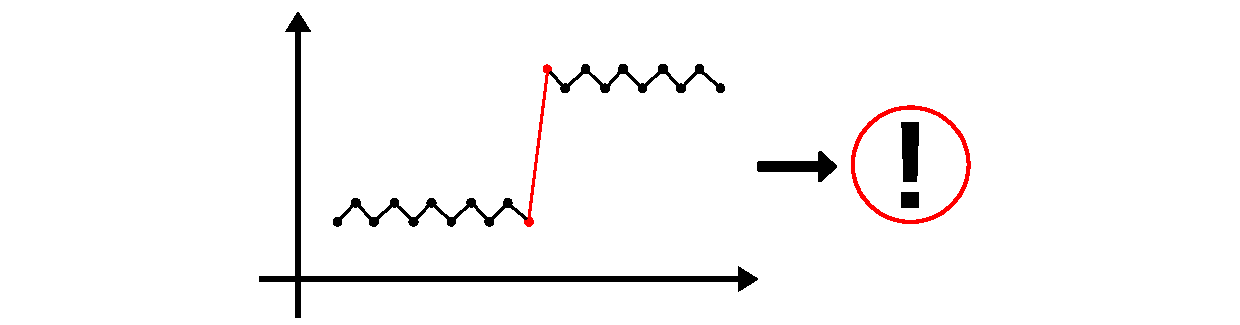
\includegraphics[width=1\textwidth]{Model update process Detection}
\caption[Model update process: Change Detection]{Change Detection: system KPIs are monitored; when a KPI variation occurrence is detected, it is reported for further analysis.}
\label{fig:Model update process Detection}
\end{figure}
\item \textbf{Change identification}\\A detected change of one or more indicators is classified to determine what kind of variation occurred in the underlying process. To do so, a “change map” is interrogated, in order to match the indicator detected change with a real system change, and then choose the correct update to the process model. Figure \ref{fig:Model update process Identification} schematically represents a Change Identification example.
\begin{figure}[H] 
\centering    
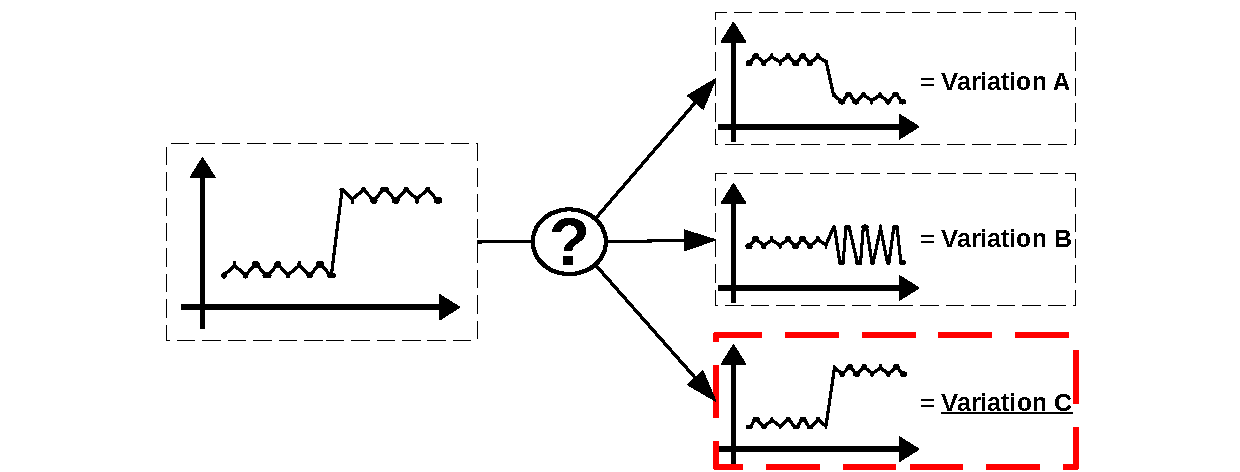
\includegraphics[width=1\textwidth]{Model update process Identification}
\caption[Model update process: Change Identification]{Change Identification: KPI variations are analyzed to identify the type of change occurred in the process.}
\label{fig:Model update process Identification}
\end{figure}
\item \textbf{Model modification}\\The process model is modified accordingly to the identified variation. A radical way to update the model is to build it from scratch, using PM algorithms, every time a variation occurs; however, in case of limited or local changes, it is not recommended to use this procedure, since the computational time and effort could be excessive. For this reason, a better approach could be the design of algorithms more specific to the occurring variation type and position, aiming to a more focused rather than a general change in the model. Figure \ref{fig:Model update process Modification} schematically represents a Model Modification example.
\begin{figure}[H] 
\centering    
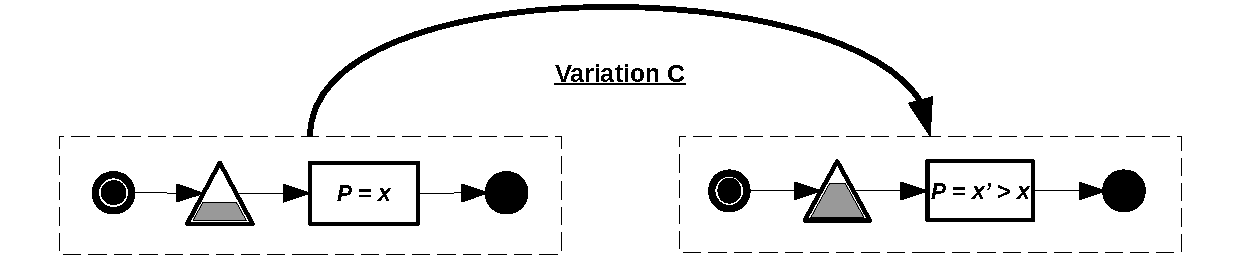
\includegraphics[width=1\textwidth]{Model update process Modification}
\caption[Model update process: Model Modification]{Model Modification: the process model is re-aligned with the real system.}
\label{fig:Model update process Modification}
\end{figure}
\end{itemize}
\subsection{Aim of the work}
\label{Aim of the work}
This thesis focuses on the second step of the model update process and, partially, on the first step. \\
Concerning the change detection, this thesis aims to answer whether or not a certain type of variation in the system is noticeable observing the monitored process indicators. Detection methods usage and even which one to apply fall outside the scope of the work. In other words, the focus is on whether a change can be detected, not on how to detect it. \\
At the same time, the thesis addresses the change identification topic, checking if it is possible to recognize the type of variation through the analysis of indicator behaviors. The main goal is to build a variation map that can be used as a guide to get insights on the process evolution. \\
This thesis is devised as part of the PM framework. In this regard, the observed indicators are extracted only from event logs generated by line sensors. The reason of this choice is to base the model update on the same data used to build the model in the first place, without requiring the addition of other sensors and the analysis of different data structures. \\
To show the novelty of this approach, the following sections are dedicated to a state of the art overview concerning the PM manufacturing applications and the PM adaptations to allow dynamic process model updates in general-purpose applications.
\section{Process Mining applications in manufacturing}
PM has been applied in manufacturing mostly as a process monitoring tool. For example, in \cite{ErMahendrawathiandArsadNovalandAstutiH.M.andPradinaRennyandUtamiRivia} PM is utilized to build the model of a production planning process of a manufacturing company using event logs obtained from an ERP system. A similar application of PM is performed in \cite{ParkMinjeongandSongMinseokandBaekTaeandSonSookyoungandHaSeungandChoSung}, where PM algorithms are adapted to analyze manufacturing make-to-order production processes, focusing on the resource workloads and on the delays caused by issues during the process. It is to be noted that, even if these studies are conducted in manufacturing contexts, they do not actually examine production lines, rather they use PM to analyze the manufacturing systems on a production planning level, and therefore are quite far from the PM application this thesis aims to achieve. \\
Lugaresi et al. in \cite{LugaresiG.2019MsmG}, as previously outlined, instead direct their attention on designing a PM algorithm which can be applied on production lines, in order to easily and swiftly build a DT imitating a real system. The mining procedure presented in the article consists of four steps:
\begin{enumerate}
\item Dataset loading: an event log is pre-filtered and pre-processed to generate the data structures suitable for the information extraction.
\item Optimized mining of event types: this is the core of the procedure, consisting in the application to data of the PM algorithm adapted to production line applications in order to obtain an \textit{activity network}, which shows how activities are connected in the system.
\item Petri Net model generation: the \textit{activity network} is translated in an initial Petri Net model\footnote{Petri Nets are process modelling language}.
\item Petri Net model adjustment: the initial Petri Net Model is polished to obtain a formally correct Petri Net model representing the real system.
\end{enumerate}
Therefore, the article shows that it is possible to mine the necessary information from a system event log to generate a process model, which can serve as a DT logical base. This thesis inserts on the same line of research, aiming to develop around this method and suggesting a procedure to move from a DT one-off generation to an always up-to-date DT.
\section{Auto-update of process models using Process Mining}
\label{Auto-update of process models using Process Mining}
In real applications, event logs often do not present as complete datasets, instead they are generated continuously appending new events recorded in real-time. In other words, an event stream is collected in an always-extending event log and there is no point in time where the dataset is finished, including the entirety of occurred events. A real-time event gathering causes challenges that basic PM algorithms are not able to deal with, since they require datasets to be finite. The PM branch that aims to address this problem is called Streaming Process Discovery (SPD), and different solutions have been developed, such as the usage of smarter forms of sampling, and summarizing the data into event frequency tables. \\
The main issue to confront when dealing with event stream is the occurrence of variations in the real system during the process. In \cite{6900341} three algorithms are proposed, aiming to build a process model from an event stream and keeping it synchronized with the system. These algorithms are based on the \textit{Heuristic Miner}, one of the most used control-flow discovery algorithms. In \cite{7376771} a similar technique is applied, introducing a growing and pruning mechanism in order to align the \textit{prefix-tree} representing the activity relationships with the real process. A different approach is taken by \cite{DennoPeterandDickersonCharlesandHardingJennifer}, where a mixed technique is designed using probabilistic neural nets and a genetic algorithm to identify and keep updated a process model with a real manufacturing system. \\
The model updating processes designed by these articles are much different from the one this thesis suggests. Indeed, in these methods models are influenced by every single event occurring in the system, without an actual monitoring of the process; instead, the approach we propose is based on the detection (and identification) of variations to trigger the model updates. Here the thesis originality lies: before model modifications we think it is critical to understand if and what kind of change is verifying in the real process, in order to minimize the updating computational effort and to be able to build a DT on more stable and reliable process models.
